\section{CORE Design}
\begin{figure}[htbp]
    \centering
    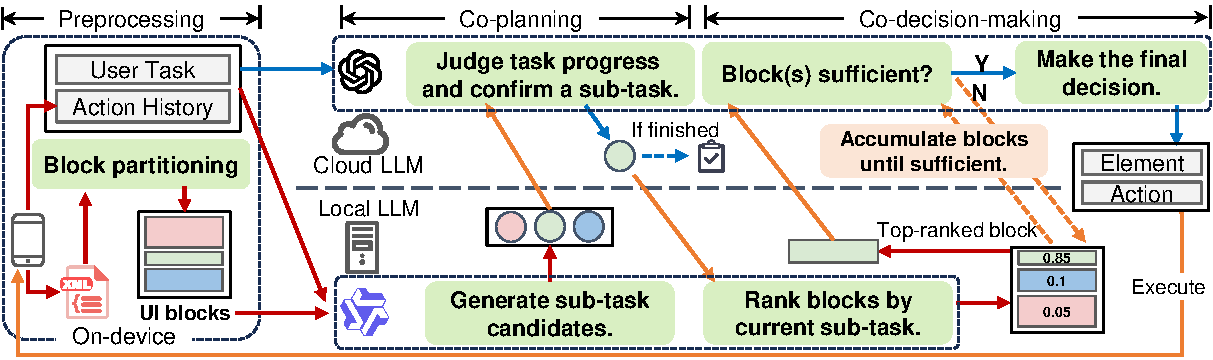
\includegraphics[width=1\textwidth]{pics/method_pipeline_v3.pdf}
    \caption{Overview of our \textbf{CORE} pipeline. It has three stages: on-device pre-processing, co-planning, and co-decision-making. In the latter two stages, it leverages the cloud LLM's strength of strong reasoning abilities and the local LLM's strength of full access to the UI blocks to collaborate.}
    \label{fig:pipeline}
    \vspace{-3mm}
\end{figure}
The design goal is to upload only sufficient UI content to the cloud, minimizing unnecessary information exposure while maintaining task performance. To this end, we propose a collaborative framework CORE that leverages the cloud LLM's strong reasoning capabilities and the local LLM's full access to the UI context. CORE consists of three stages: the \textit{on-device preprocessing stage} takes the XML screen as input and divides UI elements into semantically coherent blocks \(B_t\); the \textit{collaborative planning stage} takes the task \(T\), history \(H_t\), and blocks \(B_t\) (accessible only to the local LLM) to determine the current sub-task \(s^*\); and the \textit{collaborative decision-making stage} takes \(T\), \(H_t\), \(s^*\), and subset of \(B_t\) to output a device-executable decision \(D_t\), specifying the target UI element and action. Figure~\ref{fig:pipeline} illustrates the pipeline; further details are provided below.
\subsection{Layout-aware Block Partitioning}
Current XML-based mobile agents convert the screen represented by XML file into a simplified HTML-style UI elements list \(X_t\) so that LLMs can better understand, with each element like <button text="Add" description="Add alarm" index=2>. The drawbacks are that the list of elements becomes lengthy on complex screens, and the structural relationships implied by the original XML layout are ignored. Actually, these UI elements can be naturally grouped into several coarse-grained blocks based on the XML tree structure. Therefore, we propose a layout-aware block partitioning strategy. 

A depth-first search is applied to extract important UI elements (e.g. clickable and containing some semantics, editable) from the XML tree, which follows the traditional processing. However, unlike prior works, during traversal, we assign each node a unique index and record the ancestor path $A(x) = [a_0, a_1, \dots, a_{k-1}]$ of every important node $x \in X_t$ , where $a_0$ is the root's index and $a_{k-1}$ is the index of $x$'s parent. Many unimportant nodes skipped during traditional processing (e.g., layout containers like \texttt{FrameLayout}) act as shared ancestors of multiple important elements. The elements under the same ancestor container node are more likely to belong to the same logical or visual region due to the UI layout design. Given all ancestor paths $\{A(x)\}$, we traverse the ancestor levels from depth $i = 0$ up to the maximum path length $k_{\text{max}} - 1$. At each level $i$, we partition important elements into different blocks by their different $i$-th ancestor $a_i$, where elements under the same $a_i$ are grouped in the same block. This produces block partitions of varying granularity, coarser at shallower levels (e.g., $i = 0$ yields a single block), and finer at deeper levels (e.g., $i = k_{\text{max}} - 1$ yields the most blocks). We select the first level $i$ where the partition results in at least 3 distinct blocks, and return the blocks as the final layout-aware grouping. A toy example is shown in Figure~\ref{fig:blockpartition}.\footnote{We simplify the XML tree in Figure~\ref{fig:blockpartition} for illustration by removing or merging some nodes.}

\begin{figure}[htbp]
    \centering
    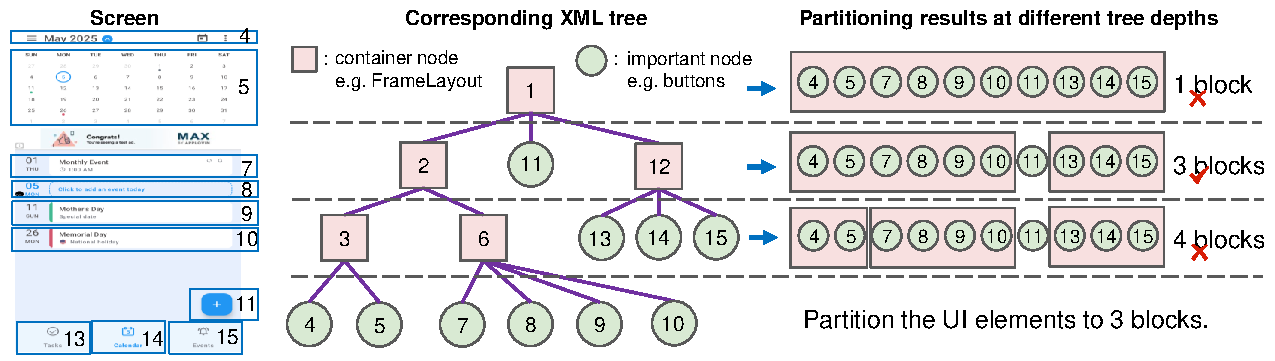
\includegraphics[width=1\textwidth]{pics/method_block_partitioin_v2.pdf}
    \caption{Our layout-ware block partitioning on a Calendar page. By comparing the ancestors of all important nodes at the same tree depth, we group them into blocks. Different depths yield different partition granularities; we select a suitable one to obtain 3 coherent blocks.}
    \label{fig:blockpartition}
    \vspace{-3mm}
\end{figure}

\subsection{Collaborative Planning}\label{cp}
The local LLM uses its access to full UI blocks to convey page understanding to the cloud LLM, which then uses superior planning skills to generate more accurate sub-tasks. We adopt a divide-and-conquer strategy to make local LLM predict the possible sub-task candidate for each UI block, as it is limited in long-context processing. For each block, we input the user-provided task description, the historical operations, and itself into the local LLM. It is required to infer and output the most reasonable sub-task that could be executed within the block without any leakage of direct element information. After processing all blocks, we aggregate the sub-tasks generated by the local LLM into a candidate set. These candidates, together with the global task description and historical operations, are then sent to the cloud LLM. The cloud LLM selects the most suitable candidate as the current sub-task, or revises/generates one if none of them is appropriate. 

The sub-task candidate derived from each block represents high-level abstractions over the block's UI elements, capturing what the local LLM considers the most important for that block. As the blocks are partitioned according to the UI’s internal logical structure, the cloud LLM can infer the rough functionalities of different blocks based on the candidate sub-tasks without access to detailed UI elements. Through comprehensive analysis of the candidate sub-tasks, the cloud LLM can piece together an approximate understanding of the overall page layout and content. This indirect perception enables the cloud LLM to make more accurate judgments about the task progress and ensures its planning remains grounded in the actual UI context.

\subsection{Collaborative Decision-making}\label{cd}
We provide the local LLM with the full set of page blocks along with the confirmed sub-task given by co-planning, and ask it to assign a score to each block based on its estimated importance for executing the sub-task. We adopt a probabilistic scoring scheme, where the local model predicts the probability that each block is useful for the current sub-task, and the scores are normalized to sum to one. This scoring produces a ranking over all blocks, reflecting the local LLM's belief about their relevance to the sub-task at the block level. The block with the highest score which is deemed most relevant and useful by the local model is then transmitted to the cloud LLM. The cloud LLM, with its stronger fine-grained reasoning capabilities, performs element-level decision-making: selecting the specific UI element to interact with and determining the action type. 

We also introduce a multi-round accumulation mechanism to handle challenging tasks requiring long context and offers fault tolerance against local filtering errors. Upon inspecting the initially provided block, the cloud LLM evaluates whether the available information is sufficient for a confident decision. If not, it requests additional blocks from the local model. The local model then selects the next most probable block among those not yet uploaded and sends it to the cloud side. The cloud model incrementally integrates the newly received block with previously accumulated information and re-evaluates the decision. This iterative process continues until the cloud model judges that it has gathered enough context to make an informed and reliable decision. By dynamically adjusting the amount of information retrieved, this mechanism strikes a balance between minimizing information upload and ensuring decision accuracy. Even if the local model initially mis-ranks blocks or provides insufficient context, the cloud model can progressively recover the necessary information through incremental retrieval, maintaining robustness against local errors and variations in task difficulty. 

\begin{wrapfigure}{r}{0.53\textwidth}
\vspace{-1.4em}
\begin{algorithm}[H]
\caption{Cloud-local collaboration at Step $t$}
\label{alg:core2e}

\KwIn{Task $T$, History $H_t = [D_1, ..., D_{t-1}]$, UI blocks $B_t = [b_1, ..., b_k]$}
\KwOut{Decision $D_t$ specifying action $a$ and target element $e$}

$S \gets [\ ]$, $C \gets [\ ]$;

\ForEach{$b_i$ \textbf{in} $B_t$}{
    $s_i \gets \text{LLM}_{\text{local}}.\text{generateSubtask}(T, H_t, b_i)$\;
    Append $s_i$ to $S$\;
}

$s^* \gets \text{LLM}_{\text{cloud}}.\text{confirmBestSubtask}(T, H_t, S)$\;

$B_{\text{ranked}} \gets \text{LLM}_{\text{local}}.\text{rank}(B_t, s^*)$\; 

\ForEach{$b$ \textbf{in} $B_{\text{ranked}}$}{
    Append $b$ to $C$\;
    $(a, e) \gets \text{LLM}_{\text{cloud}}.\text{makeDecision}(T, H_t, C)$\;
    \If{$(a, e) \ne \text{None}$}{
        \Return{$(a, e)$}
    }
}
\Return{None}
\end{algorithm}
\vspace{-6em}
\end{wrapfigure}

Algorithm~\ref{alg:core2e} summarizes the collaboration mechanism between the cloud and local models, as described in Sections~\ref{cp} and~\ref{cd}.